\documentclass[12pt]{article}
\usepackage{graphicx}
\usepackage{amsmath}
\usepackage{float}
\usepackage[]{mcode}
\usepackage{geometry}
 \geometry{
 a4paper,
 total={210mm,297mm},
 left=20mm,
 right=20mm,
 top=25mm,
 bottom=25mm,
 }
\setlength{\parindent}{0pt}
\usepackage{color}
\newcommand{\hilight}[1]{\colorbox{yellow}{#1}}
\usepackage{xcolor}
\usepackage{listings}
 
% Copied from the listings documentation
\lstdefinestyle{MyFrame}{backgroundcolor=\color{yellow},frame=shadowbox}
\lstdefinestyle{MyC++Style} {language=C++,style=MyFrame,frame=none,backgroundcolor={}}
\lstset{language=C++,frame=none}

\begin{document}

	\title{Finite Element Method for The Heat equation}
	\author{Andres Chaves(), Diego Montufar(661608)}
	
	\maketitle
	
	\begin{abstract}
		Throughout this document we are going to make use of the Finite Element Method to solve the Heat Equation that models the heat flux distribution through cooling fins on the top of a CPU.  Given the quite big amount of computation required to solve a system constructed by using this method, it's a perfect study case to apply High Performance computing tools like openMP and MPI. In this particular problem, we've implemented a matlab program and a c++ version. The domain was decomposed into tetrahedral linear elements and the time discretization was done by using the implicit Euler method. As visualization tools we used the ones provided by matlab and Paraview. Our first approach shows how a constant heat flux generated by a CPU disparses through a Box grid and then we extend that into a structured grid of the cooling fins. We tested the speedup of the implemented programs with a weak scaling methodology.
	\end{abstract}
	
	\section{Introduction}
	The Finite Element method is a powerful computational technique to solve a variety of 'real-world' engineering problems having complex domains subjected to general boundary conditions. Those domains are decomposed into simply shaped regions, or "elements". An approximate solution for the PDE can be developed for each of these elements. The total solution is then generated by linking together, or "assembling", the individual solutions taking care to ensure continuity at the interelement boundaries. Thus, the PDE is satisfied in a piecewise fashion.\\
	
Although the particulars will vary, the implementation of the finite-element approach usually follows a standard step-by-step procedure:\\

\begin{enumerate}
  \item Discretization of the domain into finite elements.
  \item Select of interpolation/shape functions
  \item Derive element matrices for the system
  \item Assembly the element matrices into a global matrix.
  \item Impose boundary conditions
  \item Compute the problem solution.
\end{enumerate}

In order to solve the Heat Equation for this particular problem we are going to derive all the equations by following the mentioned procedure and then we are going to compute and visualize the solution through the implementation of a matlab program. Our first approach involves the simulation of a heat flux constantly applied to the bottom of a 3D Box which represents what we'll later convert into a structured grid of a cooling fins on the top of a CPU. The discretization of the domain will be done by using tetrahedral linear elements. \\

Then we are going to translate our matlab code into a c++ sequential version which involves the implementation of some linear algebra operations and as we are going to store quiet big amount of data for the global systems of equations (which are represented by sparse matrices), we are going to use some implementations of code that allow us to reallocate memory when necessary by using a "Compress Row Storage" technique. The results will be visualized with Paraview throughout vtk files generated by the c++ program.\\

Once we have our sequential version of the program, the next step will be to parallelize it with an Hybrid version of the code implementing openMP for multithreading and openMPI for multiprocessor communication. This version will be run on the BlueGeneQ (Avoca) and there will be a weak scaling test in order to show the speedup results of the parallelization process.\\

Finally, we must mention that we've used as reference the code implementations from Example 15.3 and Example 21.4 taken from the Lecture's Book[1] and other resources such as unstructured grid files as well. The learning outcomes of this Assignment are the ability to apply The Finite element method to the 3D Heat equation and compute its solution using High performance computing techniques with openMP and MPI for this particular problem.\\ 
	
	\section{Problem Statement}
	
The heat equation can be used to describe the temperature variation through a
solid body. The equation derives from the principle of conservation of energy
and gives rise to a second order linear PDE of the form:
	
	\begin{equation}\label{eq:equation}
		\rho C \frac{\partial T}{\partial t} = k \nabla^2 T
	\end{equation}
	
Where $T$ is the temperature $[K]$,$\rho$ is the mass density $[kgm^3]$, $C$ is the specific heat capacity $[Jkg^{-1}K^{-1}]$, and $k$ is the thermal conductivity $[Wm^{-1}K^{-1}]$. For this particular implementation the computational domain will describe cooling fins on top of a central processing unit
and will be defined by an unstructured tetrahedral grid. We assumed that the cooling fins are made from pure copper, having the properties $\rho = 8954kgm^3$, $C = 380Jkg^{-1}K^{-1}$, and $k = 386Wm^{-1}K^{-1}$. \\

In this particular case the CPU creates a constant heat flux $Q_{cpu}$ , given by:

	\begin{equation}
		Q_{cpu} = k \nabla T
	\end{equation}
	
which defines a Neumann boundary condition on the base of the domain and $Q_{cpu} = 40,000Wm^{-2}$. For the remaining boundary of the cooling fins we assumed a convection boundary condition, given by:

	\begin{equation}
		Q_{air} = k \nabla T = h(T-T_{air})
	\end{equation}

which defines a Robin boundary condition. Here we assumed that the convection coefficient $h = 100W/m^2K^{-1}$ and the ambient temperature $T_{air} = 300K$. Defining the initial temperature of the cooling fins as ambient, the main goal is  to simulate the temperature rise in the domain $t \in [0,100]s$ and determine the maximum steady state temperature of the cooling fins.
	

%----------------------------------------------------------	
	
	\section{Governing Equations}

\subsection{Discretization of the domain into finite elements}
Weighted residual methods assume that a solution can be approximated analytically or piecewise analytically. The idea of this method is that we can multiply the residual by a weighting function and force the integral of the weighted expression over the domain to vanish:

	\begin{equation}
		\int\limits_{\Omega} W(x) r(x) d\Omega = 0
	\end{equation}
	
	We understand the residual as a continuous function of space.  In this case we are going to use the Galerking method of weighted residuals. In this method the weight functions are chosen to be identical to the trial functions where the trial function is our assumed approximate solution for the PDE which takes the form:	

	\begin{equation}
		\phi(x) = \sum_{n=0}^N a_n(x)p_n(x), \quad \text{Where}  \quad W_n(x)=p_n(x)
	\end{equation}		
	
	Applying equation (4) to the Heat Equation (1) we have:

$$
r={\rho C \frac{\partial T}{\partial t} - k \nabla^2 T}
$$

	$$\int\limits_{\Omega} W ({\rho C \frac{\partial T}{\partial t} - k \nabla^2 T}) d\Omega = 0$$
	
	This is an appropriate time to include the convection term into our equation and expanding terms we get:
	
	\begin{equation}
		\int\limits_{\Omega} W \rho C \frac{\partial T}{\partial t} d\Omega - \int\limits_{\Omega} W k \nabla^2 T d\Omega + \int\limits_{\Omega} W Q_{air} d\Omega = 0
	\end{equation}

	We can modify the diffusive second order term by applying the product rule for derivatives which is defined by:
	
\begin{align*}
\nabla\cdot(W\nabla T) &= \nabla W \cdot\nabla T+W \nabla \cdot\nabla T \\
&=\nabla W \cdot\nabla T+W \nabla^2 T
\end{align*}

In our second term of Equation (6): Applying the product rule, rearranging, and integrating over the domain we get:
		
	\begin{equation}
	\int\limits_{\Omega} W k \nabla^2 T d\Omega = \int\limits_{\Omega} \nabla \cdot ({Wk\nabla T}) d\Omega - \int\limits_{\Omega} \nabla W \cdot k \nabla T d\Omega
	\end{equation}

	in order to eliminate second order terms of the Equation (7), another important concept we are going to use is the theorem of divergence which can be expressed as follows:
	
	$$
	\int\limits_{\Omega} \nabla^22 T d\Omega = \int\limits_{\Gamma} \nabla T \cdot d\Gamma 
	$$
	
Now, we can make use of the Divergence Theorem and apply it to the second order term of Equation (7) as follows:	
	
	\begin{equation}
	\int\limits_{\Omega} k W \nabla^2 T d\Omega = \int\limits_{\Gamma} {kW\nabla T} \cdot d \mathbf{\Gamma} - \int\limits_{\Omega} k \nabla W \cdot \nabla T d\Omega
	\end{equation}

	Substitute Equation (8) in (6) we get:
	
	\begin{equation}
	\int\limits_{\Omega} \rho C W \frac{\partial T}{\partial t} d\Omega -  \int\limits_{\Gamma_{Base}} {kW\nabla T} \cdot d \mathbf{\Gamma} - \int\limits_{\Omega} k \nabla  W \cdot \nabla T d\Omega + \int\limits_{\Gamma_{Fins}} W Q_{air} d\Gamma = 0
	\end{equation}
	
	The important point here is that applying the Galerkin method of weighted residuals this way means that for every element we get a 'sub' system of equations local to each element and in terms of the local nodal values $1...N_n$, that must be assembled
into a global system of equations with global indices $1...N_p$
		
	Then we can see the second term in the equation corresponds to the value of $Q_{cpu}$ as stated in the model problem. In contrast to other methods, the Neumann boundary conditions are automatically incorporated into the integral form of the PDE. Rearranging terms we get the Weak form of the Heat Equation:

	\begin{equation}
	\int\limits_{\Omega} \rho C W \frac{\partial T}{\partial t} d\Omega + \int\limits_{\Omega} k \nabla W \cdot \nabla T d\Omega = \int\limits_{\Gamma_{Base}} {kW\nabla T} \cdot d \mathbf{\Gamma} - \int\limits_{\Gamma_{Fins}} W {h(T-T_{air})} d\Gamma
	\end{equation}

The overall global system of equations to solve our generic scalar transport equation is then given by:

	\begin{equation}
	\sum_{n=1}^{N_p}\int\limits_{\Omega} (W \rho C \frac{\partial T}{\partial t} + \nabla W \cdot k \nabla T) d\Omega = \sum_{n=1}^{N_p} \int\limits_{\Gamma_{Base}} {Wk\nabla T} \cdot d \mathbf{\Gamma} - \sum_{n=1}^{N_p} \int\limits_{\Gamma_{Fins}} W {h(T-T_{air})} d\Gamma
	\end{equation}


	\subsection{Shape functions}

One of the fundamental steps in a finite element analysis is the discretization of a continuous body containing infinite number of points in the surface into a discrete model with a limited number of points (or nodes) in the surface. The shape of the body between these nodes its approximated by functions. These functions are known as shape functions, and allow us to relate the coordinates of every point of a finite element with the positions of its nodes.

Thinking of $T$ most generally as being a continuous function of space and time, we will write the assumed solution in the form:

\begin{equation}
T(\mathbf{x},t) = \sum_{n=1}^{N_n} \eta_n(\mathbf{x})T_n(t)
\end{equation}

Where $\eta_n$ are known as the \textsl{shape functions}, which are functions of spatial location only, while the nodal values of $T$ are functions of time only. 

If we now substitute in our assumed form of the solution from Equation (10), and consider the domain of integration to be the domain of an element itself, the weighted residual expression can be rewritten using Einstein summation notation as:

	\begin{equation}
	\int\limits_{\Omega_e} \eta_p\eta_q \rho C \frac{\partial T}{\partial t} d\Omega + \int\limits_{\Omega_e} k \nabla \eta_p \cdot \nabla \eta_q T_q d\Omega = \int\limits_{\Gamma_{e}}{k\eta_p\nabla T} \cdot d \mathbf{\Gamma} - \int\limits_{\Gamma_{e}}h\eta_p(\eta_qT_q-T_{e}) d\Gamma
	\end{equation}

Then the overall System of Equations to solve the Heat Equation is the given by:

\begin{equation}
	\sum_{e=1}^{N_e}  \int\limits_{\Omega_e} \bigg(\eta_p\eta_q \rho C \frac{\partial T_q}{\partial t} d\Omega + k \nabla \eta_p \cdot \nabla \eta_q T_q\bigg) d\Omega = \sum_{e=1}^{N_e} \int\limits_{\Gamma_{e}}{k\eta_p\nabla T} \cdot d \mathbf{\Gamma} - \sum_{e=1}^{N_e} \int\limits_{\Gamma_{e}}\eta_p h (\eta_qT_q-T_{air}) d\Gamma
	\end{equation}

We can then rewrite the system of equations in the form:

\begin{equation}
 M\dot{T} = KT + s
\end{equation}

Where $M$ represents the Mass matrix, $K$ the Stiffness Matrix, both have size of $N_p$x$N_p$ and finally the $s$ term that is the load vector with size $N_p$x$1$. For the Heat Equation we can recognize each term of Equation(15) in the Equation (13) as follows:

\begin{equation}
 M_{pq}^e = \int\limits_{\Omega_e} \rho C \eta_p\eta_q  d\Omega
\end{equation}

\begin{equation}
 K_{pq}^e = - k \int\limits_{\Omega_e} \nabla \eta_p \cdot \nabla \eta_q d\Omega - h \int\limits_{\Gamma_e} \eta_p \eta_q d\Gamma
\end{equation}

\begin{equation}
 S_{p}^e = h T_{air} \int\limits_{\Gamma_e} \eta_p d\Gamma + k \int\limits_{\Gamma_{e}}{\eta_p\nabla T} \cdot d \mathbf{\Gamma}
\end{equation}

For this case we are going to use tetrahedral elements, which means we are going to have 4 nodes in a 3D \hilight{element as shown in Figure()}. In order to derive the corresponding shape functions we begin by assuming a trial solution which takes the form:

\begin{equation}
T(x,y,z) = a_0+a_1x+a_2y+a_3z
\end{equation}

Where $a_0$,$a_1$,$a_2$ and $a_3$ are scalar coefficients. This is essentially the 3D equivalent of the trial solution to a triangular element. If we apply this trial solution in every node of the element we'll get:

\begin{equation}
\begin{Bmatrix} T_1 \\ T_2 \\ T_3 \\ T_4 \end{Bmatrix} = 
\begin{bmatrix} 1 & x_1 & y_1 & z_1 \\ 1 & x_2 & y_2 & z_2 \\ 1 & x_3 & y_3 & z_3 \\ 1 & x_4 & y_4 & z_4\end{bmatrix}
\begin{Bmatrix} a_0 \\ a_1 \\ a_2 \\ a_3 \end{Bmatrix} =
\begin{bmatrix} \mathbf{p_1} \\ \mathbf{p_2} \\ \mathbf{p_3} \\ \mathbf{p_4} \end{bmatrix}\mathbf{a} = C\mathbf{a}
\end{equation}

Where $p_n=\{1 \thinspace x_n \thinspace y_n \thinspace z_n\}$, $C$ will be a square $4$x$4$ matrix and we can solve for the unknown parameters by computing $\mathbf{a}=C^{-1}\mathbf{T}$. Doing so we can find our shape functions by substituting these coefficients back into our trial solution, So we can factor out the nodal values and rewrite the solution in the form:

\begin{equation}
T(x,y,z) = \sum_{n=1}^{N_n} \eta_n{(x,y,z)} T_n = \eta_1 T_1 + \eta_2 T_2 + \eta_3 T_3 + \eta_4 T_4
\end{equation}

Where the shape functions for the linear tetrahedron are:

\begin{center}
  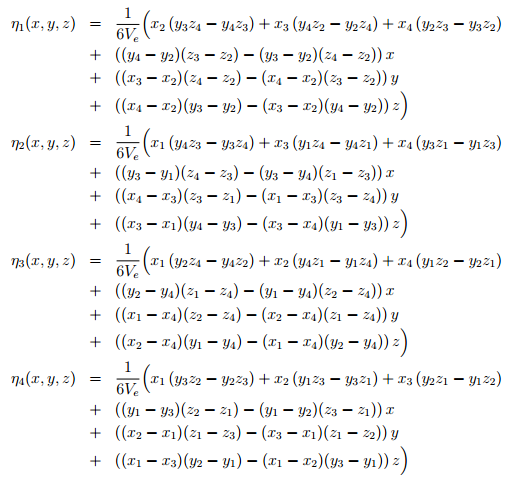
\includegraphics[width=0.8\textwidth]{ShapeFunctions}
\end{center}

Where $V_e$ is the volume of the element and is defined in terms of its nodal coordinates as:

\begin{equation}
6V_e=\begin{bmatrix} 1 & x_1 & y_1 & z_1  \\ 1 & x_2 & y_2 & z_2  \\ 1 & x_3 & y_3 & z_3 \\ 1 & x_4 & y_4 & z_4 \end{bmatrix}
\end{equation}

And we could express the derivatives of the shape functions as:

\begin{center}
  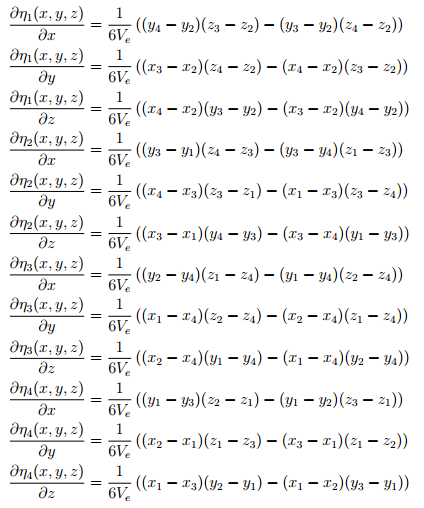
\includegraphics[width=0.7\textwidth]{GradientShapeFunctions}
\end{center}

Furthermore, we have the integration formulae defined for the linear tetrahedron:

\begin{equation}
 \int\limits_{\Omega_e} \eta_p^a \eta_q^b \eta_r^c \eta_s^d d{\Omega}=
 \frac{a!b!c!d!6\Omega_e}{(a+b+c+d+3)!}
\end{equation}

and:

\begin{equation}
 \int\limits_{\Gamma_e} \eta_p^a \eta_q^b \eta_r^c  d{\Omega}=
 \frac{a!b!c!2\Gamma_e}{(a+b+c+2)!}
\end{equation}

Where for the 3D case $\Omega_e$ and $\Gamma_e$ represent the volume and face area of a tetrahedron respectively.

\subsection{Derive element matrices for the System}


Let's first consider the integration of the shape functions as required in the mass matrix from Equation (16):

$$
M_{p,q}^e = \rho C \int\limits_{\Omega_e} \eta_p \eta_q d\Omega
$$

Remembering that p and q are in the range of 1 to 4 for the linear tetrahedral element,
what we end up with is a local or 'sub' matrix $M_e$, which for our linear tetrahedral
element will be a 4 x 4 matrix. In order to evaluate each term in the matrix we
simply input the values of p and q to the integration formula in Equation (23). For
the case where p and q are equal (i.e. for elements on the main diagonal) we get:

\begin{align*}
 M_{p,p}^e & = \rho C  \int\limits_{\Omega_e} \eta_p \eta_p d\Omega \\
              	& = \rho C \int\limits_{\Omega_e} \eta_p^2 \eta_q^0 \eta_r^0 \eta_s^0 d{\Omega}=
 \frac{\rho C 2!0!0!0!6\Omega_e}{(2+0+0+0+3)!} \\
 				& = \frac{2\rho C \Omega_e}{20}
\end{align*}

For the case where p and q are not equal (i.e. for elements off the main diagonal) we get:

\begin{align*}
 M_{p,q}^e & = \rho C \int\limits_{\Omega_e} \eta_p \eta_q d\Omega \\
              	& = \rho C \int\limits_{\Omega_e} \eta_p^1 \eta_q^1 \eta_r^0 \eta_s^0 d{\Omega}=
 \frac{\rho C 1!1!0!0!6\Omega_e}{(1+1+0+0+3)!} \\
 				& = \frac{\rho C \Omega_e}{20}
\end{align*}

So we can write a single expression for the any element in our local mass matrix as:

$$
M_{p,q}^e = \frac{\rho C (1+\delta_{pq})}{20}
$$

which is simple enough that we could write out the whole thing as:

\begin{equation}
M^e = \frac{\rho C \Omega_e}{20}{\begin{bmatrix} 2 & 1 & 1 & 1 \\ 1 & 2 & 1 & 1 \\ 1 & 1 & 2 & 1 \\ 1 & 1 & 1 & 2 \end{bmatrix}}
\end{equation}

Considering now the contribution of the diffusive term to the stiffness matrix, and writing shape function derivative terms in the form of a column vector with modulo 3 notation for compactness we have:


\begin{align*}
 -k\int\limits_{\Omega_e} \nabla \eta_p \cdot \nabla \eta_q d\Omega &= \\ 
 &= -k\int\limits_{\Omega_e} \frac{1}{6\Omega_e} 
 \begin{Bmatrix} 
 (y_{p+3}-y_{p+1})(z_{p+2}-z_{p+1})-(y_{p+2}-y_{p+1})(z_{p+3}-z_{p+1}) \\
 (x_{p+2}-x_{p+1})(z_{p+3}-z_{p+1})-(x_{p+3}-x_{p+1})(z_{p+2}-z_{p+1}) \\
 (x_{p+3}-x_{p+1})(y_{p+2}-y_{p+1})-(x_{p+2}-x_{p+1})(y_{p+3}-y_{p+1}) \\
 \cdots
 \end{Bmatrix} \\
 &\dot{•} 
 \frac{1}{6\Omega_e} 
 \begin{Bmatrix} 
 (y_{q+3}-y_{q+1})(z_{q+2}-z_{q+1})-(y_{q+2}-y_{q+1})(z_{q+3}-z_{q+1}) \\
 (x_{q+2}-x_{q+1})(z_{q+3}-z_{q+1})-(x_{q+3}-x_{q+1})(z_{q+2}-z_{q+1}) \\
 (x_{q+3}-x_{q+1})(y_{q+2}-y_{q+1})-(x_{q+2}-x_{q+1})(y_{q+3}-y_{q+1}) \\
 \cdots
 \end{Bmatrix}
\end{align*}

Performing the Integration we get:

\begin{equation}
\begin{aligned}
-k\int\limits_{\Omega_e} \nabla \eta_p \cdot \nabla \eta_q d\Omega &= \\
 & -\frac{k}{36\Omega_e^2} 
 \begin{Bmatrix} 
 (y_{p+3}-y_{p+1})(z_{p+2}-z_{p+1})-(y_{p+2}-y_{p+1})(z_{p+3}-z_{p+1}) \\
 (x_{p+2}-x_{p+1})(z_{p+3}-z_{p+1})-(x_{p+3}-x_{p+1})(z_{p+2}-z_{p+1}) \\
 (x_{p+3}-x_{p+1})(y_{p+2}-y_{p+1})-(x_{p+2}-x_{p+1})(y_{p+3}-y_{p+1}) \\
 \cdots
 \end{Bmatrix} \\
 &\dot{•} 
 \begin{Bmatrix} 
 (y_{q+3}-y_{q+1})(z_{q+2}-z_{q+1})-(y_{q+2}-y_{q+1})(z_{q+3}-z_{q+1}) \\
 (x_{q+2}-x_{q+1})(z_{q+3}-z_{q+1})-(x_{q+3}-x_{q+1})(z_{q+2}-z_{q+1}) \\
 (x_{q+3}-x_{q+1})(y_{q+2}-y_{q+1})-(x_{q+2}-x_{q+1})(y_{q+3}-y_{q+1}) \\
 \cdots
 \end{Bmatrix} {\Omega_e}
\end{aligned}
\end{equation}

The important point to note is that the dot product between these two vectors
produce a scalar value. Now we obtain the second part of the contribution to the stiffness matrix again first evaluating the integral for the main diagonal where p=q:

\begin{align*}
 -h \int\limits_{\Gamma_e} \eta_p \eta_p d\Gamma & = 
 -h\int\limits_{\Gamma_e} \eta_p^2 \eta_q^0 \eta_r^0  d{\Gamma} \\
 & = -\frac{h 2!0!0!2\Gamma_e}{(2+0+0+2)!} \\
 & = -\frac{2h\Gamma_e}{12}
\end{align*}

Then we do the same for the off diagonal terms where p $\neq$ q:

\begin{align*}
 -h \int\limits_{\Gamma_e} \eta_p \eta_q d\Gamma & = 
 -h\int\limits_{\Gamma_e} \eta_p^1 \eta_q^1 \eta_r^0  d{\Gamma} \\
 & = -\frac{h 1!1!0!2\Gamma_e}{(1+1+0+2)!} \\
 & = -\frac{h\Gamma_e}{12}
\end{align*}

So we can write a single expression for the any element in the contribution term for our local stiffness matrix as:

$$
K_{p,q}^e =- \frac{h (1+\delta_{pq})}{12}
$$

which is simple enough that we could write out the whole thing as:

\begin{equation}
K^e = -\frac{h \Gamma_e}{12}{\begin{bmatrix} 2 & 1 & 1  \\ 1 & 2 & 1  \\ 1 & 1 & 2 \end{bmatrix}}
\end{equation}

Considering the contribution of the Neumann boundary condition term to
the load vector, we have to perform the integral:

\begin{align*}
 \mathbf{s}_p^f = k \int\limits_{\Gamma_{e}}{\eta_p\nabla T} \cdot d \mathbf{\Gamma}
\end{align*}

An important point to note is that we will only perform this integral over the boundary of the element (which in our case translates into a  face of a triangle) if that element happens to be on a Neumann boundary of our computational domain. In this case p will be in the range 1 to 3. Because our Neumann boundary conditions are applied normal to the boundary, the gradient can be specified as a scalar (the implied direction being normal to the boundary face) and so the dot product will drop out of the integral. We will furthermore assume that $T$ does not vary over the boundary of the element. Making use of the second integration formula (24) we then have:

\begin{align*}
 \mathbf{s}_p^f &= k \int\limits_{\Gamma_{e}}{\eta_p\nabla T} \cdot d \mathbf{\Gamma} \\
 &= k \nabla T \int\limits_{\Gamma_{e}}{\eta_p} \cdot d \mathbf{\Gamma} \\
 &= k \nabla T \frac{h 1!0!0!2\Gamma_e}{(1+0+0+2)!} \\
 &= \frac{k\nabla T\Gamma_e}{3}
\end{align*}

So we can write the contribution to our load vector as:

\begin{equation}
\mathbf{s}_p^f = \frac{k\nabla T\Gamma_e}{3}
\begin{bmatrix} 1 \\ 1 \\ 1 \\ 1 
\end{bmatrix}
\end{equation}

And finally we obtain the first part of our load vector as follows:

\begin{align*}
 \mathbf{s}_p^e &= hT_{air} \int\limits_{\Gamma_{e}}{\eta_p} \cdot d \mathbf{\Gamma} \\
 &= hT_{air} \int\limits_{\Gamma_{e}}{\eta_p} \cdot d \mathbf{\Gamma} \\
 &= hT_{air} \frac{h 1!0!0!2\Gamma_e}{(1+0+0+2)!} \\
 &= \frac{hT_{air}\Gamma_e}{3}
\end{align*}

So we can write the contribution to our load vector as:

\begin{equation}
\mathbf{s}_p^e = \frac{hT_{air}\Gamma_e}{3}
\begin{bmatrix} 1 \\ 1 \\ 1 \\ 1 
\end{bmatrix}
\end{equation}

\subsection{Assemble}

\subsection{Apply Boundary conditions}

Robin boundary convective boundary conditions

\section{Problem Solution and Implementation}

In order to compute the solution of the problem, firstly we implemented a Matlab program using a Box grid as our first approach to test the results. Then we translated it into its c++ sequential version. At this point we'll be going to show the output results in Paraview through an unstructured Box grid as well as a more complex figure representing a CPU heat sink. After getting the desired results we are going to parallelize the sequential version of the c++ code by using MPI and openMP.

\subsection{Matlab and C++ implementation}
As we are going to reuse the code provided in the Lectures and tutorials, we decided to describe only the part of the code that was modified/added and some relevant comments related to it. For this part of the implementation we used the \textit{Example21-4.m} for the matlab code and \textit{Example21-4.cpp} for the c++ sequential version. The domain will be in $x\in[0,0.02]$, $y\in[0,0.02]$, $z\in[0,0.02]$ and $t\epsilon[0,100]$. For the spatial discretization we will use the Finite Element method with linear tetrahedral elements, for the temporal discretization we will use the implicit Euler method, and we will solve the resulting linear system with the Conjugate Gradient method. The first step is to set up all the constant terms from the Heat equation. This could be done by adding the next lines:

\begin{lstlisting}
rho            = 8954.00;
C              = 380.00;
k              = 386.00;
h              = 100.00;
Tair           = 300.00;
Qcpu           = 40000.00;
\end{lstlisting}

In c++ we could do the similar:

\begin{lstlisting}[style=MyC++Style]
const double rho            = 8954.00;
const double C              = 380.00;
const double k              = 386.00;
const double h              = 100.00;
const double Tair           = 300.00;
const double Qcpu           = 40000.00;
\end{lstlisting}

As mentioned in the problem statement, we assumed the initial temperature of the cooling fins as ambient (300K). Thus we set the initial condition as follows:

\begin{lstlisting}
% Set initial condition
phi(:,1)        = 300;
\end{lstlisting}

And in the c++ version:

\begin{lstlisting}[style=MyC++Style]
for(int m=0; m<N_p; m++){
	phi[m]	= 300;
}
\end{lstlisting}

In Matlab the read function is defined to return the value and number of the Points, Faces, Elements and Boundaries defined in the grid file. This file contains pretty exactly the same for both Matlab and c++ programs, the only difference is that Matlab will 'automatically' set the parameter values in structs and vector variables and the c++ program has to go through the file line by line, so that it can dynamically allocate the required memory and will also 'know' how many of each entity to read in. An example of a grid file is shown as follows:

\begin{lstlisting}
N_p = 812;
N_f = 1244;
N_e = 2949;
N_b = 2;
Points = [
0.00000	0.00000	0.00000
0.00000	0.02000	0.00000
0.02000	0.02000	0.00000
...
];
Faces = [
     9	    10	   185
     9	   155	     1
     9	   185	   155
...
];
Elements = [
   574	   544	   556	   757
   686	   133	   169	   740
   237	   725	   240	   754
...
];
Boundaries = struct('name',{},'type',{},'N',{},'indices',{},'value',{});
Boundaries(1).name    = 'Fins';
Boundaries(1).type    = 'robin';
Boundaries(1).N       = 1050;
Boundaries(1).indices = [ 1 2 3 4 5 6 7 8 9 10 11 12 13 14 15 16 17 ... ];
Boundaries(1).value   = 0.00000;
...
\end{lstlisting}

The \textit{read} function for the c++ version was modified in order to get the data for the linear tetrahedron elements defined in the grid file. This file could be a simple Box grid or a more complex form like a CPU sink. We will be storing three arrays for this problem; an array called Points which is an $N_p$x$3$ array storing the x, y and z coordinates of the points defining the grid, an array called Faces which is an $N_f$x$3$ array storing the three indices of the points defining a face in the grid, and an array called Elements which is an $N_e$x$4$ array storing the three indices of the points defining an element in the grid, we can see this definitions in the following code:

\begin{lstlisting}[style=MyC++Style]
file >> temp >> N_p;
file >> temp >> N_f;
file >> temp >> N_e;
file >> temp >> N_b;

Points			= new double*	[N_p];
Faces			= new int*		[N_f];
Elements		= new int*		[N_e];
Boundaries		= new Boundary  [N_b];
Points[0]       = new double    [N_p*3];
Faces[0]        = new int       [N_f*3];
Elements[0]     = new int       [N_e*4];
\end{lstlisting}

Where "file" is the fstream object which handles the input file, the "temp" variable will be used to read and store some 'useless' data from the file (i.e. the description labels for each value), All the arrays to store Points, Faces and Elements, and finally a "Boundaries" variable which is an instance of the \textit{Boundary} class. 
\\\\
At this point we should mention that Matlab allow us to perform basic linear algebra operations very easily with matrices and structs, however, we cannot do exactly the same with c++. As we are going to store and compute a quite big amount of data, specially when we are dealing with the global system of equations after the assemble process, we are going to make use of the provided \textit{SparseMatrix} and \textit{Boundary} class definitions as 'includes' in our c++ program. The first one handles basic operations between matrices like sums, subtracts, multiplications, etc. And the second one is a basic data structure to store all the information related to Boundaries defined on each grid file. 
\\\\
Now we have all the variables ready to load all the data from the input files, and this can be done simply by looping over each parameter and structure defined in the file as follows:

\begin{lstlisting}[style=MyC++Style]
file >> temp;
for(int p=0; p<N_p; p++){
	file >> Points[p][0] >> Points[p][1] >> Points[p][2];
}

file >> temp;
for(int f=0; f<N_f; f++){
	file >> Faces[f][0] >> Faces[f][1] >> Faces[f][2];
}

file >> temp;
for(int e=0; e<N_e; e++){
	file >> Elements[e][0] >> Elements[e][1] >> Elements[e][2] >> Elements[e][3];
}
\end{lstlisting}

At this point we can apply the spatial discretization that is the Finite Element method to our PDE. We know that we will have a discrete system which takes the form $M\dot{T} = KT + s$ with each element matrix and load vectors defined in Equation 16,17 and 18 respectively, with that in mind now we are going to compute all those local element matrices by using the derivations performed in part 3.3.
\\\\
To assemble these matrices we are going to need to evaluate $\Omega_e$ and $\Gamma_f$ for the elements and faces respectively. Now in this case for the 3D Heat Equation $\Omega_e$ is the volume of each tetrahedron, which we can evaluate in matlab as:

\begin{lstlisting}
% Calculate element volumes
for e=1:N_e	
	x           = Points(Elements(e, :), 1);
	y           = Points(Elements(e, :), 2);
	z           = Points(Elements(e, :), 3);
	Omega(e)	= abs(    x(1)*y(2)*z(3) - x(1)*y(3)*z(2) - x(2)*y(1)*z(3) ...
						+ x(2)*y(3)*z(1) + x(3)*y(1)*z(2) - x(3)*y(2)*z(1) ...
						- x(1)*y(2)*z(4) + x(1)*y(4)*z(2) + x(2)*y(1)*z(4) ...
						- x(2)*y(4)*z(1) - x(4)*y(1)*z(2) + x(4)*y(2)*z(1) ...
						+ x(1)*y(3)*z(4) - x(1)*y(4)*z(3) - x(3)*y(1)*z(4) ...
						+ x(3)*y(4)*z(1) + x(4)*y(1)*z(3) - x(4)*y(3)*z(1) ...
						- x(2)*y(3)*z(4) + x(2)*y(4)*z(3) + x(3)*y(2)*z(4) ...
						- x(3)*y(4)*z(2) - x(4)*y(2)*z(3) + x(4)*y(3)*z(2) ) /6;
end
\end{lstlisting}

And the c++ version which looks similar for that part would be:

\begin{lstlisting}[style=MyC++Style]
for(int e=0; e<N_e; e++){
	for(int p=0; p<4; p++){
		x[p]	= Points[Elements[e][p]][0];
		y[p]	= Points[Elements[e][p]][1];
		z[p]	= Points[Elements[e][p]][2];
	}
	Omega[e]    = abs(x[0]*y[1]*z[2] - x[0]*y[2]*z[1] - x[1]*y[0]*z[2]
				 + x[1]*y[2]*z[0] + x[2]*y[0]*z[1] - x[2]*y[1]*z[0]
				 - x[0]*y[1]*z[3] + x[0]*y[3]*z[1] + x[1]*y[0]*z[3]
				 - x[1]*y[3]*z[0] - x[3]*y[0]*z[1] + x[3]*y[1]*z[0]
				 + x[0]*y[2]*z[3] - x[0]*y[3]*z[2] - x[2]*y[0]*z[3]
				 + x[2]*y[3]*z[0] + x[3]*y[0]*z[2] - x[3]*y[2]*z[0]
				 - x[1]*y[2]*z[3] + x[1]*y[3]*z[2] + x[2]*y[1]*z[3]
				 - x[2]*y[3]*z[1] - x[3]*y[1]*z[2] + x[3]*y[2]*z[1]) /6;
}
\end{lstlisting}

In 3D $\Gamma_f$ is a face area of a triangular element and we can compute this in matlab quite simply via:

\begin{lstlisting}
% Calculate face areas
for f=1:N_f	
	x           = Points(Faces(f, :), 1);
	y           = Points(Faces(f, :), 2);
	z           = Points(Faces(f, :), 3);
	Gamma(f)	= sqrt(((y(2)-y(1))*(z(3)-z(1)) - (z(2)-z(1))*(y(3)-y(1)))^2 ... 
	   + ((z(2)-z(1))*(x(3)-x(1)) - (x(2)-x(1))*(z(3)-z(1)))^2 ...
	   + ((x(2)-x(1))*(y(3)-y(1)) - (y(2)-y(1))*(x(3)-x(1)))^2)/2;
end
\end{lstlisting}

And in c++ we have:

\begin{lstlisting}[style=MyC++Style]
for(int f=0; f<N_f; f++){
	for(int p=0; p<3; p++){
		x[p]	= Points[Faces[f][p]][0];
		y[p]	= Points[Faces[f][p]][1];
		z[p]	= Points[Faces[f][p]][2];
	}
	Gamma[f]	= sqrt(pow(((y[1]-y[0])*(z[2]-z[0]) - (z[1]-z[0])*(y[2]-y[0])),2)
				+ pow(((z[1]-z[0])*(x[2]-x[0]) - (x[1]-x[0])*(z[2]-z[0])),2)
				+ pow(((x[1]-x[0])*(y[2]-y[0]) - (y[1]-y[0])*(x[2]-x[0])),2))/2;
}
\end{lstlisting}

The next step is to loop over the nodes of an element and evaluate the terms in the local mass matrix, stiffness matrix and the load vector. An important point to note here is that all the contributions to the load vector correspond to boundary values as well as the second term of the stiffness matrix and they will be considered later when we in fact will be computing the Boundaries. \cite{Steve13}
\\\\
Now in order to actually implement this in our Matlab code, our assemble function is going to involve 'looping' over all of
the elements in the grid, then looping over all of the nodes of each element. The code will look something like:

\begin{lstlisting}
...
M_e             = [2, 1, 1, 1; 
                   1, 2, 1, 1;
                   1, 1, 2, 1;
                   1, 1, 2, 1];
...
% Assemble M, K, and s
    for e=1:N_e
	
	Nodes       = Elements(e,:);
	x           = Points(Nodes,1);
	y           = Points(Nodes,2);
	z           = Points(Nodes,3);
	gradEta  	= [((y(4)-y(2))*(z(3)-z(2))-(y(3)-y(2))*(z(4)-z(2))), 
				 ((y(3)-y(1))*(z(4)-z(3))-(y(3)-y(4))*(z(1)-z(3))), 
				 ((y(2)-y(4))*(z(1)-z(4))-(y(1)-y(4))*(z(2)-z(4))), 
				 ((y(1)-y(3))*(z(2)-z(1))-(y(1)-y(2))*(z(3)-z(1)));
				 ((x(3)-x(2))*(z(4)-z(2))-(x(4)-x(2))*(z(3)-z(2))), 
				 ((x(4)-x(3))*(z(3)-z(1))-(x(1)-x(3))*(z(3)-z(4))), 
				 ((x(1)-x(4))*(z(2)-z(4))-(x(2)-x(4))*(z(1)-z(4))), 
				 ((x(2)-x(1))*(z(1)-z(3))-(x(3)-x(1))*(z(1)-z(2)));
				 ((x(4)-x(2))*(y(3)-y(2))-(x(3)-x(2))*(y(4)-y(2))), 
				 ((x(3)-x(1))*(y(4)-y(3))-(x(3)-x(4))*(y(1)-y(3))), 
				 ((x(2)-x(4))*(y(1)-y(4))-(x(1)-x(4))*(y(2)-y(4))), 
				 ((x(1)-x(3))*(y(2)-y(1))-(x(1)-x(2))*(y(3)-y(1)))]/(6*Omega(e)); 
	for p=1:4
		m               = Nodes(p);
		for q=1:4 
			n           = Nodes(q);
			gradEta_q   = [gradEta(1,q), gradEta(2,q), gradEta(3,q)];
							
			M(m,n)      = M(m,n) + rho*C*M_e(p,q)*Omega(e)/20;
			K(m,n)       = K(m,n) - k*dot(gradEta_p,gradEta_q)*(Omega(e));
		end
	end
end
\end{lstlisting}

As we can see is quite easy to compute the mass matrix and the corresponding contribution to the stiffness matrix as well. The analogous c++ version of that code looks like this: 

\begin{lstlisting}[style=MyC++Style]
...
//The Mass element Matrix
double	M_e[4][4]	= {{2.0, 1.0, 1.0, 1.0}, 
						{1.0, 2.0, 1.0, 1.0}, 
						{1.0, 1.0, 2.0, 1.0}, 
						{1.0, 1.0, 1.0, 2.0}};
...
// Assemble M, K, and s
M.initialize(N_p, 10);
K.initialize(N_p, 10);

for(int e=0; e<N_e; e++){
	for(int p=0; p<4; p++){
		Nodes[p]= Elements[e][p];
		x[p]	= Points[Nodes[p]][0];
		y[p]	= Points[Nodes[p]][1];
		z[p]	= Points[Nodes[p]][2]; 
	}

	gradEta[0][0] = ((y[3]-y[1])*(z[2]-z[1])-(y[2]-y[1])*(z[3]-z[1]))/(6*Omega[e]);
	gradEta[0][1] = ((y[2]-y[0])*(z[3]-z[2])-(y[2]-y[3])*(z[0]-z[2]))/(6*Omega[e]);
	gradEta[0][2] = ((y[1]-y[3])*(z[0]-z[3])-(y[0]-y[3])*(z[1]-z[3]))/(6*Omega[e]);
	gradEta[0][3] = ((y[0]-y[2])*(z[1]-z[0])-(y[0]-y[1])*(z[2]-z[0]))/(6*Omega[e]);
	gradEta[1][0] = ((x[2]-x[1])*(z[3]-z[1])-(x[3]-x[1])*(z[2]-z[1]))/(6*Omega[e]);
	gradEta[1][1] = ((x[3]-x[2])*(z[2]-z[0])-(x[0]-x[2])*(z[2]-z[3]))/(6*Omega[e]);
	gradEta[1][2] = ((x[0]-x[3])*(z[1]-z[3])-(x[1]-x[3])*(z[0]-z[3]))/(6*Omega[e]);
	gradEta[1][3] = ((x[1]-x[0])*(z[0]-z[2])-(x[2]-x[0])*(z[0]-z[1]))/(6*Omega[e]);
	gradEta[2][0] = ((x[3]-x[1])*(y[2]-y[1])-(x[2]-x[1])*(y[3]-y[1]))/(6*Omega[e]);
	gradEta[2][1] = ((x[2]-x[0])*(y[3]-y[2])-(x[2]-x[3])*(y[0]-y[2]))/(6*Omega[e]);
	gradEta[2][2] = ((x[1]-x[3])*(y[0]-y[3])-(x[0]-x[3])*(y[1]-y[3]))/(6*Omega[e]);
	gradEta[2][3] = ((x[0]-x[2])*(y[1]-y[0])-(x[0]-x[1])*(y[2]-y[0]))/(6*Omega[e]);

	// Outer loop over each node
	for(int p=0; p<4; p++){
		m		= Nodes[p];
		gradEta_p[0]	= gradEta[0][p];
		gradEta_p[1]	= gradEta[1][p];
		gradEta_p[2]	= gradEta[2][p];

		// Inner loop over each node
		for(int q=0; q<4; q++){
			n			= Nodes[q];
			gradEta_q[0]		= gradEta[0][q];
			gradEta_q[1]		= gradEta[1][q];
			gradEta_q[2]		= gradEta[2][q];

			M(m,n)	   += rho*C*M_e[p][q]*Omega[e]/20;
			K(m,n)	   -= k*(gradEta_p[0]*gradEta_q[0]
			+gradEta_p[1]*gradEta_q[1]
			+gradEta_p[2]*gradEta_q[2])*Omega[e];
		}
	}
}
\end{lstlisting}

Here we are computing matrices $M$ and $K$, both are instances of the \textit{SparseMatrix} class, thus we can make use of all the defined operations (methods) of that class, in fact, we are initializing the matrices in order to start assigning values to them and also computing some matrix operations like the dot product of the gradients on the right hand side of the $K(m,n)$ matrix calculation. The only thing to keep in mind is that in our c++ version we should remember that we need to initialize the \textit{SparseMatrix} objects, assemble the coefficients with the overloaded () operator, then finalize them, that could be easily done like we were using Matlab style code.
\\\\
Now it's time to compute the Boundary conditions. If we are dealing with a Robin boundaries, then indices indicates to which points in the Points array the given boundary condition needs to be applied. If however, we are dealing with a Neumann boundary, then indices indicates to which faces in the Faces array the integration of the Neumann boundary condition needs to be performed. So in this case as we mention earlier, for the Robin boundaries we are going to compute the contribution to the load vector and the contribution to the stiffness matrix with the integration performed in the first and second term of Equation (18) respectively. Then we'll do the same with the second term of Equation (17), which corresponds to the Neumann boundary condition. We can do this by adding in another for loop over the boundaries within our Matlab assemble function as:

\begin{lstlisting}
...
k_e             =   [2, 1, 1; 
                     1, 2, 1;
                     1, 1, 2];                   
s_e             = [1; 1; 1; 1];
...
% Apply boundary conditions
Fixed = [];
for b=1:N_b  
	if  strcmp(Boundaries(b).type, 'neumann')
		for f=1:Boundaries(b).N;
			Nodes       = Faces(Boundaries(b).indices(f),:);
			for p=1:3
				m     	= Nodes(p);
				%second term contribution to the load vector
				s(m)	= s(m)+ s_e(p)*Qcpu*Gamma(Boundaries(b).indices(f))/3; 
				
			end
		end        
	elseif strcmp(Boundaries(b).type, 'robin')
	   for f=1:Boundaries(b).N;
			Nodes       = Faces(Boundaries(b).indices(f),:);
			for p=1:3
				m     	= Nodes(p);
				%first term contribution to the load vector
				s(m)	= s(m)+ s_e(p)*h*Tair*Gamma(Boundaries(b).indices(f))/3; 
				for q=1:3
					n = Nodes(q);
					%Contribution to the stiffness  matrix
					K(m,n)=K(m,n)-h*k_e(p,q)*Gamma(Boundaries(b).indices(f))/12; 
				end
			end
	   end
	end
	Free = [1:N_p];
end
\end{lstlisting}

Where the Free vector is indicating all of the interior Neumann and Robin boundary points where we don't actually know the values of $T$ and the Fixed vector is indicating all of the Dirichlet boundary points where we do. In this case we don't have Dirichlet boundary conditions so in fact all the points will be assigned to the Free vector. The c++ version of the algorithm will look something like:

\begin{lstlisting}[style=MyC++Style]
...
//The contribution to the Stiffness Matrix
double	k_e[3][3]	= {{2.0, 1.0, 1.0}, 
						{1.0, 2.0, 1.0}, 
						{1.0, 1.0, 2.0}};
//The contribution to the Load vector
double	s_e[4]		= {1.0, 1.0, 1.0, 1.0};
...
//Apply Boundary Conditions
for(int b=0; b<N_b; b++){
	if		(Boundaries[b].type_=="neumann"){
		for(int f=0; f<Boundaries[b].N_; f++){
			for(int p=0; p<3; p++){
				Nodes[p]	= Faces[Boundaries[b].indices_[f]][p];
				m			= Nodes[p];
				//second term contribution to the load vector
				s[m]	   += s_e[p]*Qcpu*Gamma[Boundaries[b].indices_[f]]/3; 
			}
		}
	}
	else if	(Boundaries[b].type_=="robin"){
		for(int f=0; f<Boundaries[b].N_; f++){
			for(int p=0; p<3; p++){
				Nodes[p]	= Faces[Boundaries[b].indices_[f]][p];
				m			= Nodes[p];
				//second term contribution to the load vector
				s[m]	   += s_e[p]*h*Tair*Gamma[Boundaries[b].indices_[f]]/3; 
				 for (int q=0; q<3; q++){
					 Nodes[q]	= Faces[Boundaries[b].indices_[f]][q];
					 n = Nodes[q];
					 //Contribution to the stiffness matrix
					 K(m,n)    -= h*k_e[p][q]*Gamma[Boundaries[b].indices_[f]]/12; 
				 }
			}
			Free[m] = true;
		}
	}
}
K.finalize();
M.finalize();
\end{lstlisting}

Now the final step is the solution of our global assembled system, and we will be partitioning the matrix such that we have: 

$$
A_{Free,Free}T_{Free}^{l+1}=\textbf{b}_{Free}-A_{Free,Fixed}T_{Free}^{l+1}
$$

And so we solve a reduced system of equations and with Matlab this could be done as follows:

\begin{lstlisting}
phi(Free,l+1) = A(Free,Free)\(b(Free) - A(Free,Fixed)*phi(Fixed,l+1));
\end{lstlisting}

Where \textit{phi} is the general name of our field variable $T$. Here we will only compute the solution for the interior points and so as long as the Robin boundary points are initialized correctly in phi, then we will have imposed
the boundary conditions correctly. Now that we have shown how we assemble our system of equations, we are now in a position to write out the core of the program as:

\begin{lstlisting}
...
A = M - Delta_t*K;
...
% Time marching loop
for l=1:N_t-1
	
	b = M*phi(:,l) + Delta_t*s;
	phi(Free,l+1)	= A(Free,Free)\(b(Free) - A(Free,Fixed)*phi(Fixed,l+1));
	
	% Plot phi at every timestep
    set(Solution, 'CData', phi(:,l+1));
    title(['t = ' num2str(t(l+1))]);
    drawnow;
end
\end{lstlisting}

If we want to show the results in Matlab, we can do it by updating a Figure inside the time marching loop. At this point we can compute the maximum steady state temperature of the Box grid after 100s which is: 342.427K. The complete Matlab program is given in \textit{Assignment2.m} and the final results obtained with the simulations of our Matlab program are shown on Figure \ref{fig:matlab1}. Further captures are shown in \textbf{APPENDIX A}.

\begin{figure}[h!]
    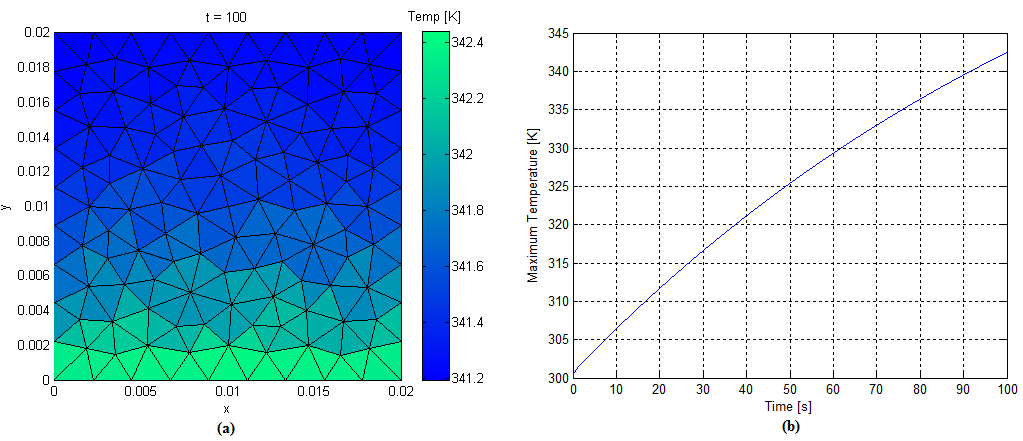
\includegraphics[scale=0.6]{matlab1}
    \caption{Figure (1.a) Heat flux trough an unstructured Box grid using linear tetrahedral elements. Figure (1.b) Maximum temperature after 100s}
    \label{fig:matlab1}
\end{figure}

For our c++ version the time marching loop will be a little bit more complex since we don't have the backslash operator to perform matrix operations easily. So we are going to explain the most relevant parts of the following code:

\begin{lstlisting}[style=MyC++Style] 
1. A = M;
2. A.subtract(Delta_t, K); // At this point we have A = M-Delta_t*K
3.
4. // Compute the column vector to subtract 
5. //from the right hand side to take account of fixed nodes
6. A.multiply(AphiFixed, phi, Free, Fixed);
7.
8. writeData(phi, Points, Elements, N_p, N_e, 0);
9. 
10. // Time marching loop
11. for(int l=0; l<N_t-1; l++){
12.	// Assemble b
13.	M.multiply(b, phi);
14.	for(int m=0; m<N_p; m++){
15.		b[m]	+= Delta_t*s[m] - AphiFixed[m];
16.	}
17.
18.	// Solve the linear system
19.	solve(A, phi, b, Free, Fixed);
20.
21.	// Write the solution
22.	if (l%10==0){
23.	   writeData(phi, Points, Elements, N_p, N_e, (l+1));
24.	}
25.}
\end{lstlisting}




\subsection{Parallel MPI C++ implementation}

\subsection{Hybrid openMP and MPI implementation}


%----------------------------------------------------------
	
	\section{Discussion}
	Write your Discussion here.	
	
	\section{Results}
	Write your Results here.
	
%		\begin{figure}
%		\centering
%		\includegraphics[width=3.0in]{myfigure}
%		\caption{Simulation Results}
%		\label{simulationfigure}
%	\end{figure}
	
	\section{Appendices}
	
	\textbf{APPENDIX A.} Matlab simulation on a Box grid with Finite Element Method for linear 3D tetrahedral elements and Implicit Euler Method.
	
	\begin{figure}[H]
    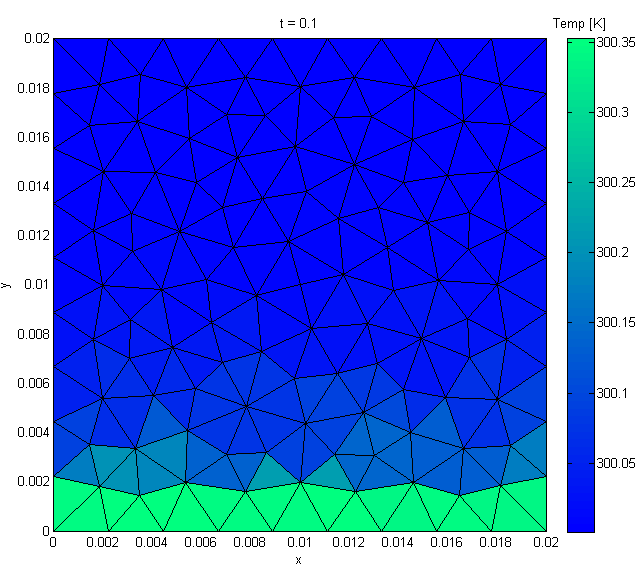
\includegraphics[scale=0.5]{matlab-results/1.png}
    \centering
    \caption{Initial state of Temperature}
	\end{figure}	
	\begin{figure}[H]
    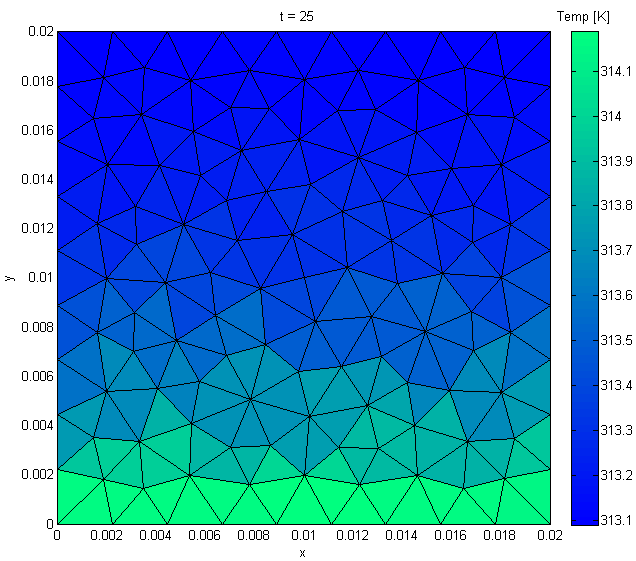
\includegraphics[scale=0.5]{matlab-results/2.png}
    \centering
    \caption{Temperature after 25 time step}
	\end{figure}	
	\begin{figure}[H]
    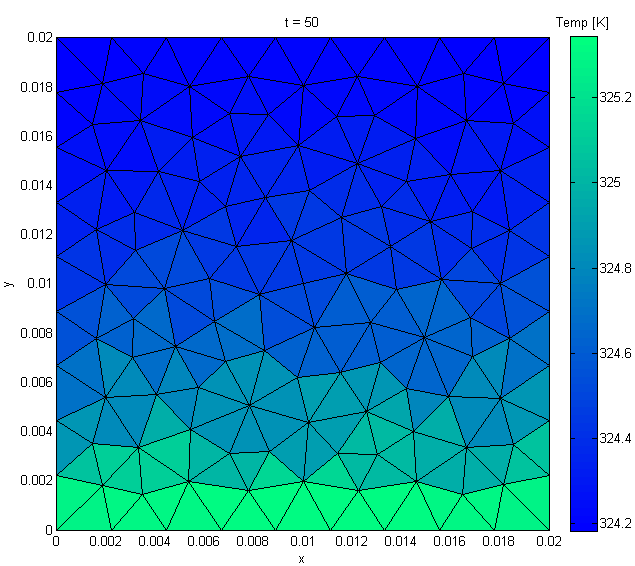
\includegraphics[scale=0.5]{matlab-results/3.png}
    \centering
    \caption{Temperature after 50 time steps}
	\end{figure}	
	\begin{figure}[H]
    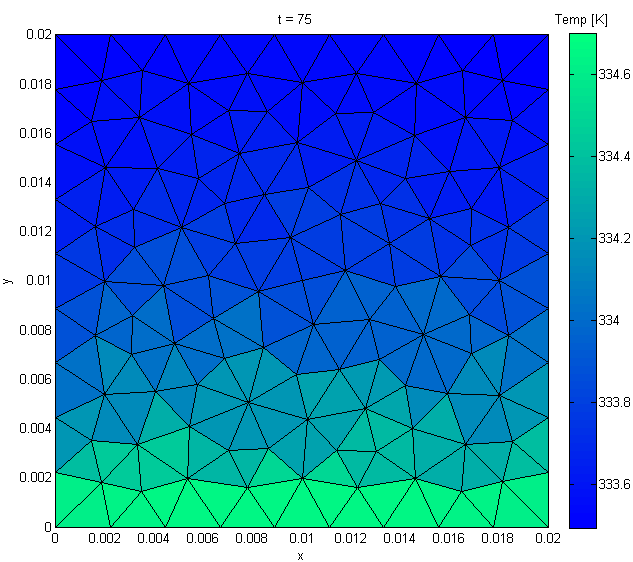
\includegraphics[scale=0.5]{matlab-results/4.png}
    \centering
    \caption{Temperature after 75 time steps}
	\end{figure}	
	\begin{figure}[H]
    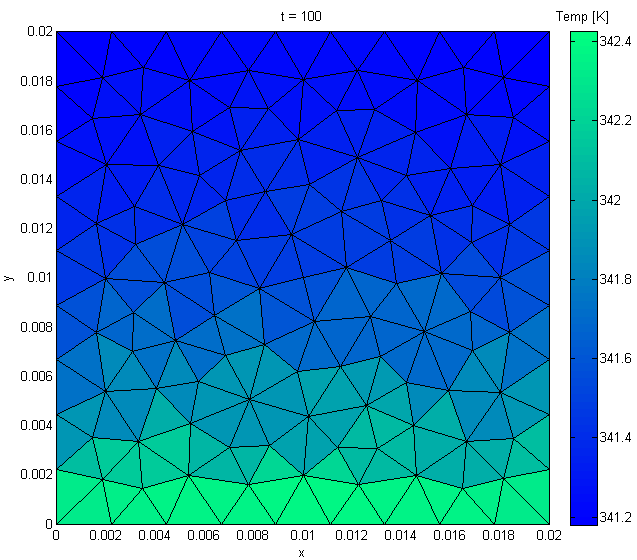
\includegraphics[scale=0.5]{matlab-results/5.png}
    \centering
    \caption{Temperature after 100 time steps}
	\end{figure}	
	\begin{figure}[H]
    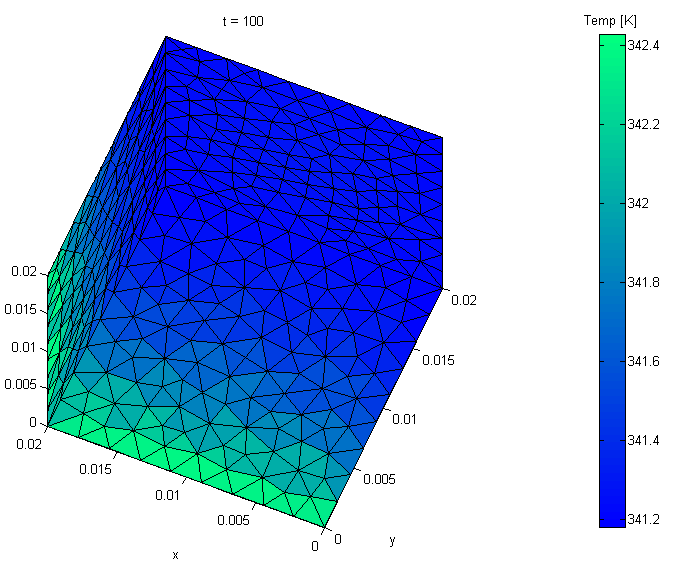
\includegraphics[scale=0.5]{matlab-results/7.png}
    \centering
    \caption{Temperature after 100 time steps, 3D Box perspective}
	\end{figure}	

	
\textbf{APPENDIX B.} c++ sequential simulation on a Box grid with Finite Element Method for linear 3D tetrahedral elements and Implicit Euler Method.
	
	\begin{figure}[H]
    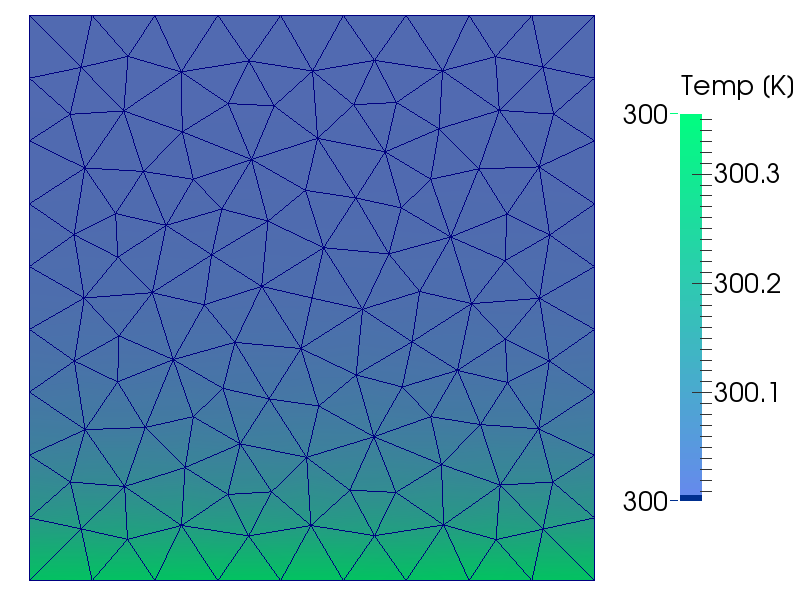
\includegraphics[scale=0.4]{box-sequential/boxSequential_ts1.png}
    \centering
    \caption{Initial state of Temperature}
	\end{figure}	
	\begin{figure}[H]
    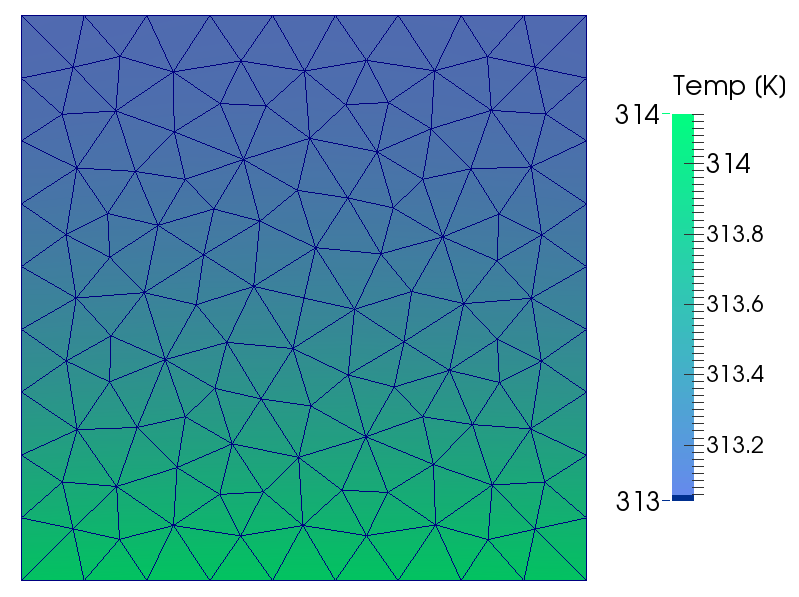
\includegraphics[scale=0.4]{box-sequential/boxSequential_ts25.png}
    \centering
    \caption{Temperature after 25 time step}
	\end{figure}	
	\begin{figure}[H]
    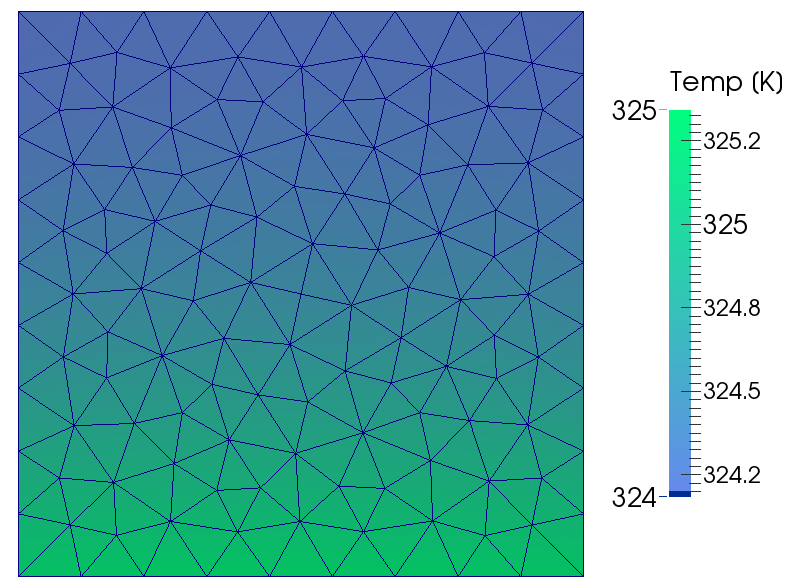
\includegraphics[scale=0.4]{box-sequential/boxSequential_ts50.png}
    \centering
    \caption{Temperature after 50 time steps}
	\end{figure}	
	\begin{figure}[H]
    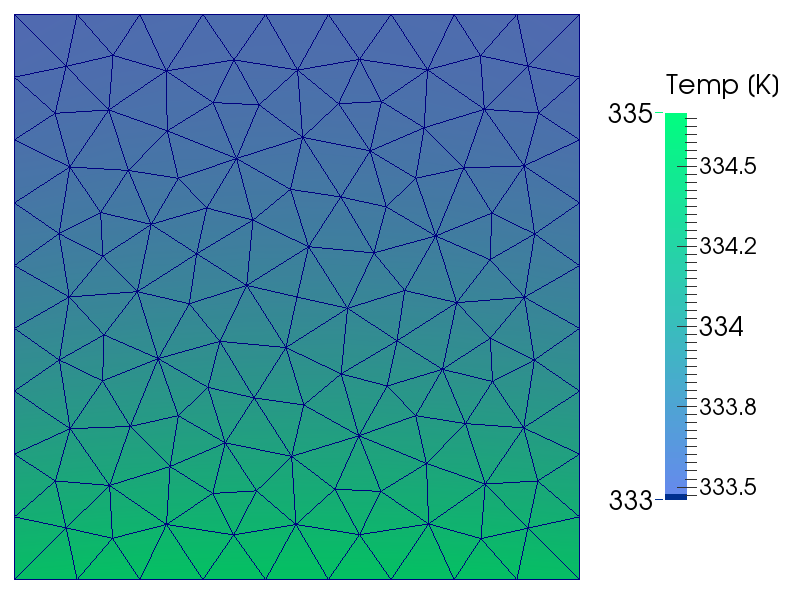
\includegraphics[scale=0.4]{box-sequential/boxSequential_ts75.png}
    \centering
    \caption{Temperature after 75 time steps}
	\end{figure}	
	\begin{figure}[H]
    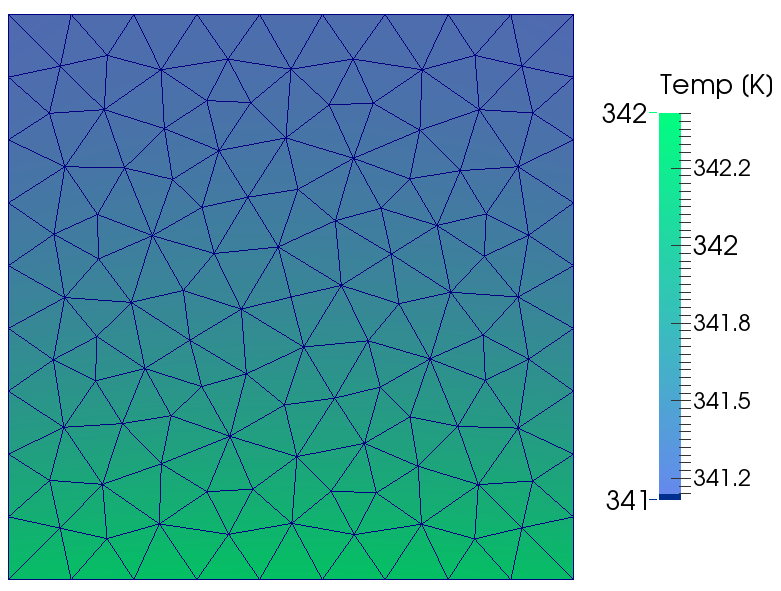
\includegraphics[scale=0.4]{box-sequential/boxSequential_ts100.png}
    \centering
    \caption{Temperature after 100 time steps}
	\end{figure}	
	\begin{figure}[H]
    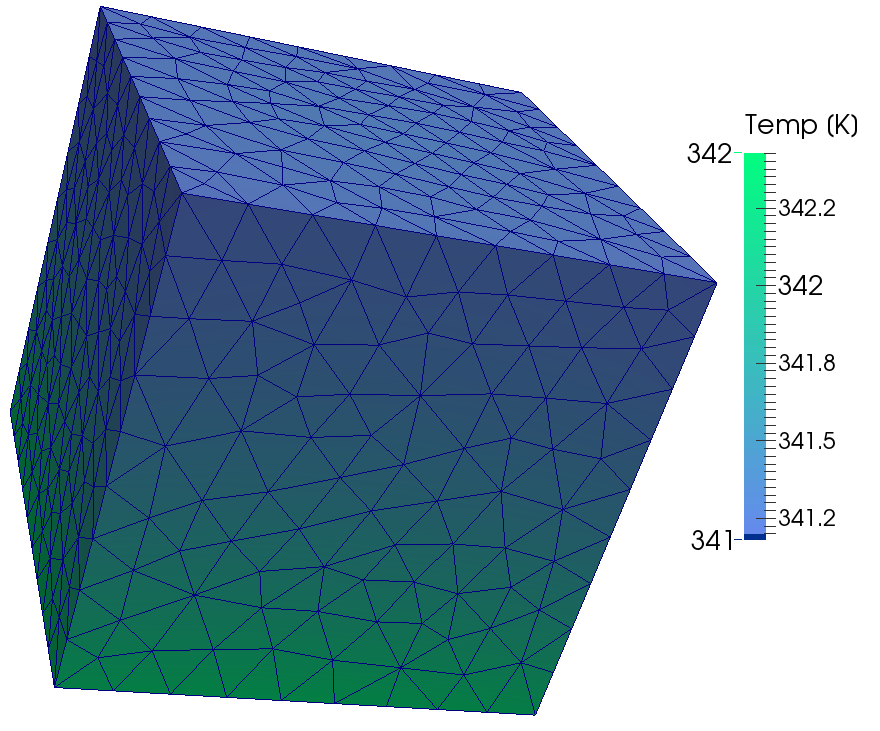
\includegraphics[scale=0.3]{box-sequential/box3dview.png}
    \centering
    \caption{Temperature after 100 time steps, 3D Box perspective}
	\end{figure}	

\textbf{APPENDIX C.} c++ Hybrid simulation on a CPU sink grid with Finite Element Method for linear 3D tetrahedral elements and Implicit Euler Method.
	
	\begin{figure}[H]
    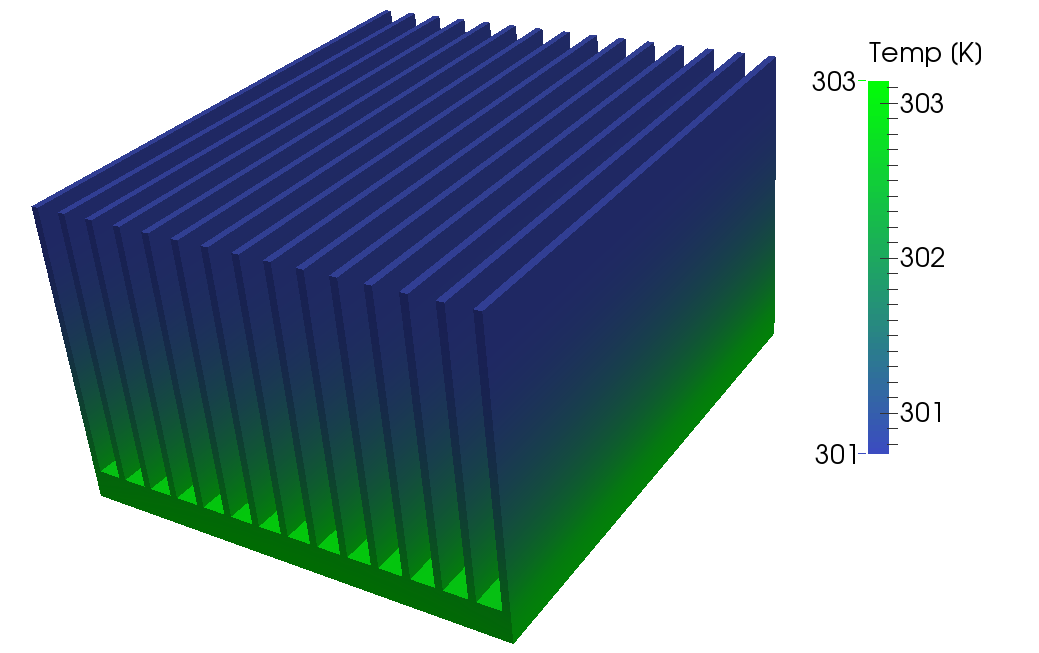
\includegraphics[scale=0.3]{sink-MPI/heatSink_mpi_ts1.png}
    \centering
    \caption{Initial state of Temperature}
	\end{figure}	
	\begin{figure}[H]
    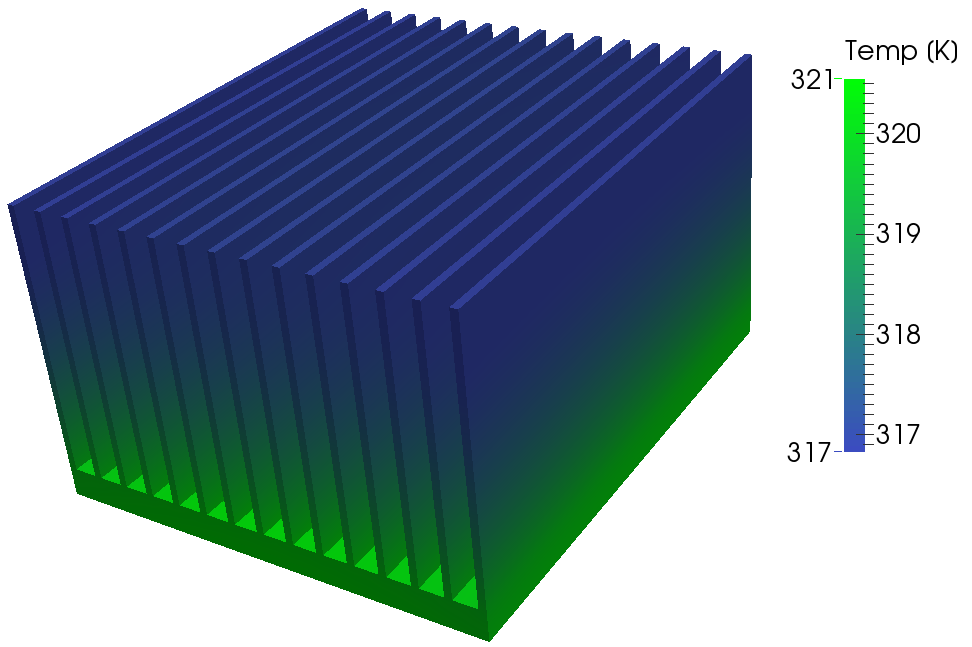
\includegraphics[scale=0.3]{sink-MPI/heatSink_mpi_ts25.png}
    \centering
    \caption{Temperature after 25 time step}
	\end{figure}	
	\begin{figure}[H]
    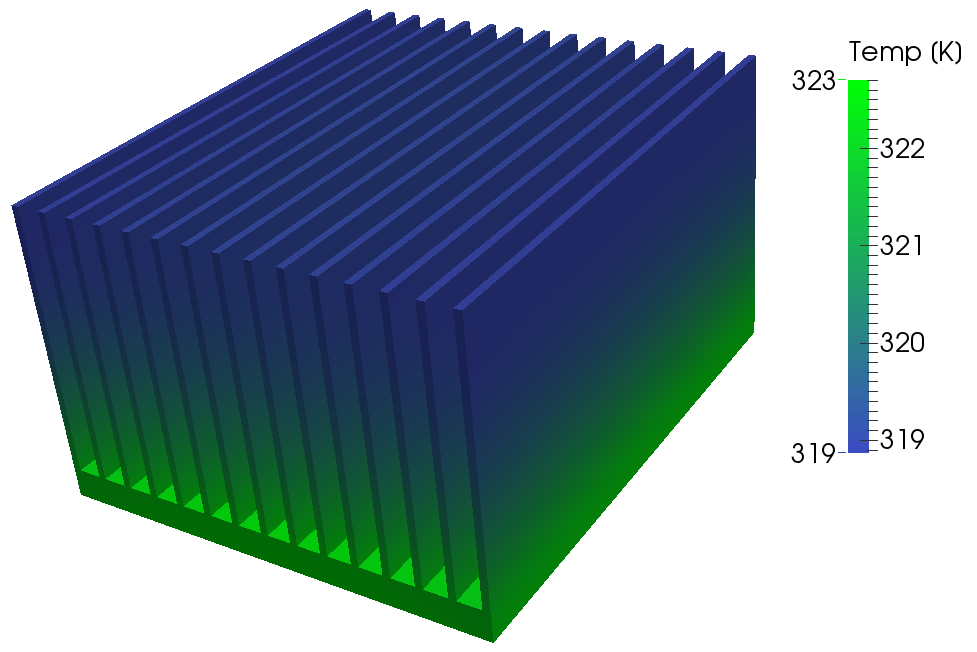
\includegraphics[scale=0.3]{sink-MPI/heatSink_mpi_ts50.png}
    \centering
    \caption{Temperature after 50 time steps}
	\end{figure}	
	\begin{figure}[H]
    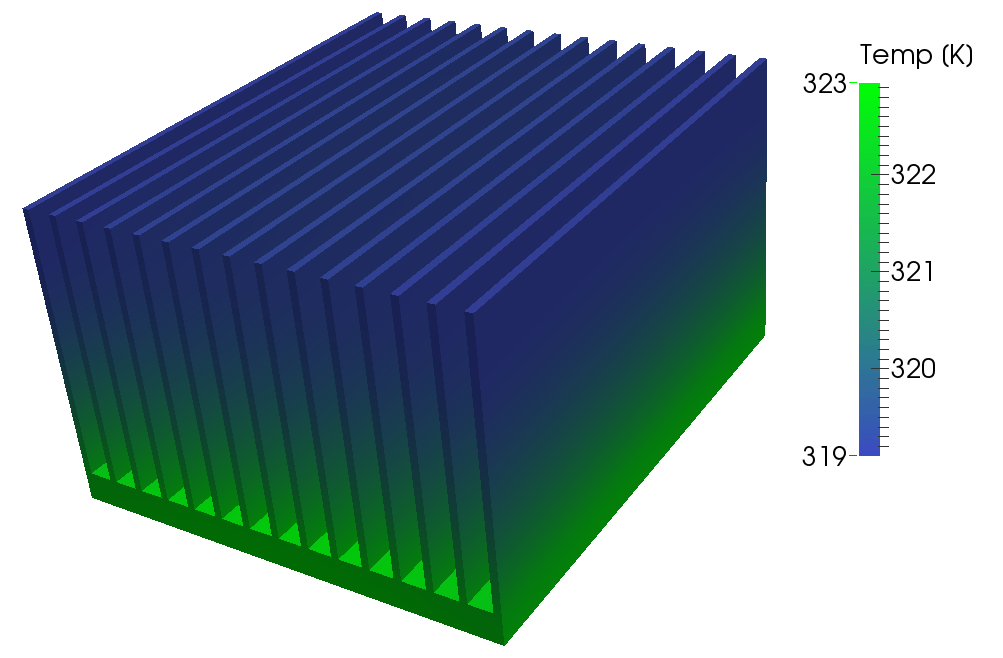
\includegraphics[scale=0.3]{sink-MPI/heatSink_mpi_ts75.png}
    \centering
    \caption{Temperature after 75 time steps}
	\end{figure}	
	\begin{figure}[H]
    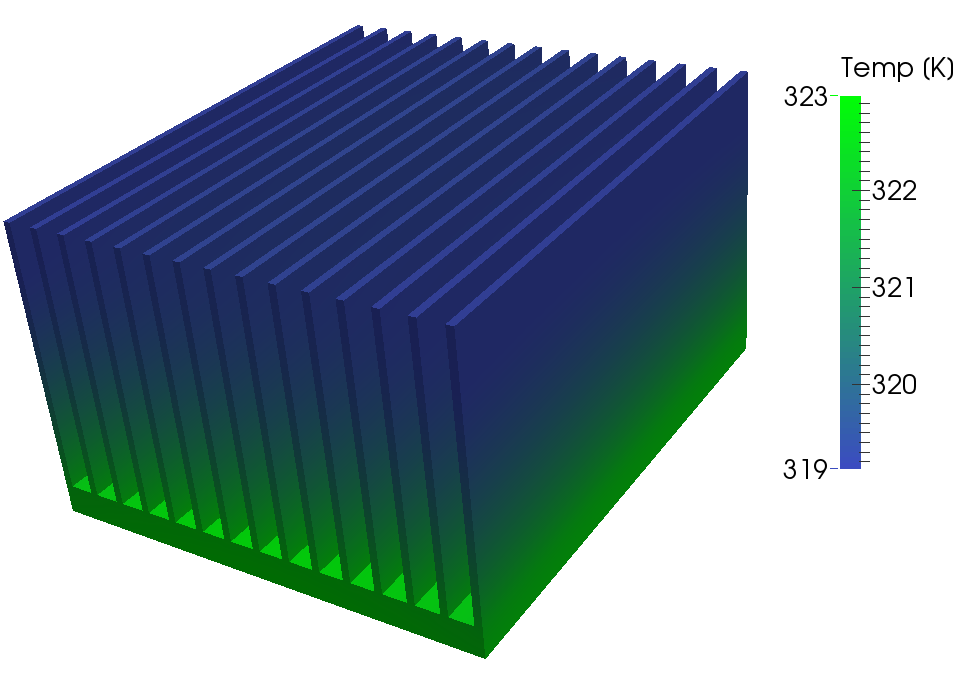
\includegraphics[scale=0.3]{sink-MPI/heatSink_mpi_ts99.png}
    \centering
    \caption{Temperature after 100 time steps}
	\end{figure}	

	\section{References}
	
	
	\bibliographystyle{amsplain}
	\bibliography{references}
	
	
	
\end{document}